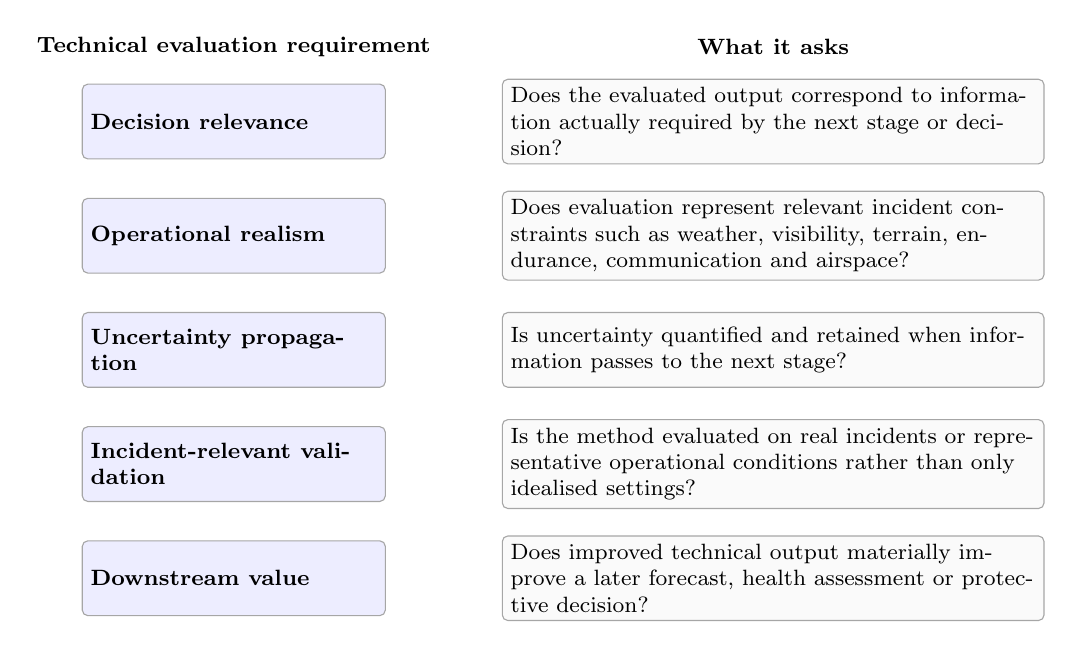
\begin{tikzpicture}[
row/.style={draw=black!35,rounded corners=2pt,minimum height=9.5mm,inner sep=3pt,font=\footnotesize,text=black},
req/.style={row,fill=blue!7,align=left,text width=0.30\linewidth,font=\bfseries\footnotesize},
meaning/.style={row,fill=black!2,align=left,text width=0.55\linewidth},
head/.style={font=\bfseries\footnotesize,text=black}
]
\node[head] at (2.1,0.45) {Technical evaluation requirement};
\node[head] at (8.95,0.45) {What it asks};
\node[req] (r1) at (2.1,-0.5) {Decision relevance};
\node[meaning] (m1) at (8.95,-0.5) {Does the evaluated output correspond to information actually required by the next stage or decision?};
\node[req] (r2) at (2.1,-1.95) {Operational realism};
\node[meaning] (m2) at (8.95,-1.95) {Does evaluation represent relevant incident constraints such as weather, visibility, terrain, endurance, communication and airspace?};
\node[req] (r3) at (2.1,-3.40) {Uncertainty propagation};
\node[meaning] (m3) at (8.95,-3.40) {Is uncertainty quantified and retained when information passes to the next stage?};
\node[req] (r4) at (2.1,-4.85) {Incident-relevant validation};
\node[meaning] (m4) at (8.95,-4.85) {Is the method evaluated on real incidents or representative operational conditions rather than only idealised settings?};
\node[req] (r5) at (2.1,-6.30) {Downstream value};
\node[meaning] (m5) at (8.95,-6.30) {Does improved technical output materially improve a later forecast, health assessment or protective decision?};
\end{tikzpicture}
